\section{Introduction}
\label{s:secIntroCMS}
\begin{figure}
  \begin{center}
  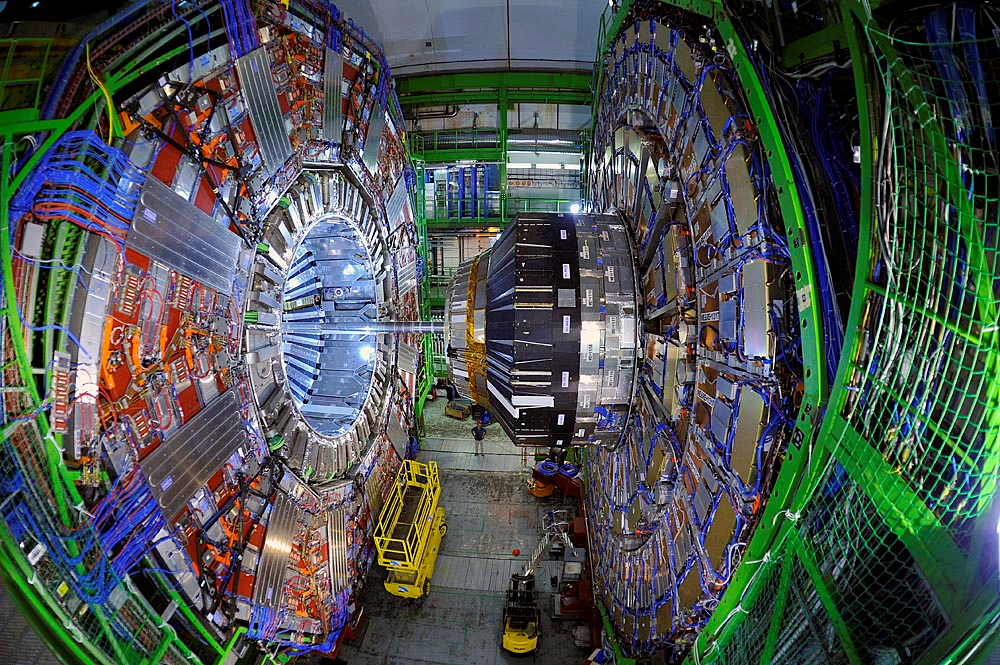
\includegraphics[width=0.90\linewidth]{Experiment/CMS/Image/cms.png}
  \caption{The CMS detector installed in IR5 at the LHC~\cite{Collaboration_2008_CMS}.}
  \label{fig:cms_exp}
  \end{center}
\end{figure}
The Compact Muon Solenoid (CMS) detector is installed in IR5 at the LHC ring. 
CMS is one of the biggest international collaborations involving 43 countries, 
199 institutes, with around 4000 people. The weight of the CMS detector is about 
14000 tonnes (around the weight of 2500 African elephants). Such a huge weight is 
accommodated in a small volume (the shape of CMS is cylindrical with length of 
21.5\unit{m}, and diameter of 15.6\unit{m}). That is why the \dq{compact} word has been 
attached to it. One of the main physics goals of the CMS experiment is to detect \dq{muons} 
as they are produced in most of the Standard Model processes. Of course, other particles 
such as an electron, photon, neutral and charged hadrons are also detected. A huge 
\dq{solenoid} magnet is placed inside the CMS to bend the tracks of charged particles so that 
their momentum can be measured precisely. An image of the CMS experiment is shown
in Figure~\ref{fig:cms_exp}, while various parts of the detectors are shown in Figure
\ref{fig:cms_diag}. The beam axis is along the center of the cylinder. The 
tracker (silicon pixel and strip) is the first sub-detector followed by the 
electromagnetic calorimeter (ECAL), and the hadron calorimeter (HCAL). The
magnetic solenoid is placed outside the HCAL followed by the muon chambers.
The iron yoke provides stand for the muon chambers and contains the magnetic 
flux outside the solenoid. A detailed description of each 
sub-detector is given in the next sections. 

The trajectories of various particles inside the CMS detector are shown in Figure
\ref{fig:cms_track}. The particles are produced at the IP and
move towards various layers of the detector. The charged particles are bent
thanks to the presence of a strong magnetic field inside the solenoid. Outside of it, 
the charged particles are bent in the opposite direction. On the other hand, the neutral particles 
do not bend inside the detector. The particles detected by the CMS experiment are 
muon, electron, charged hadron (e.g. pion), neutral hadron (e.g. neutron), and photon.
\begin{figure}
  \begin{center}
  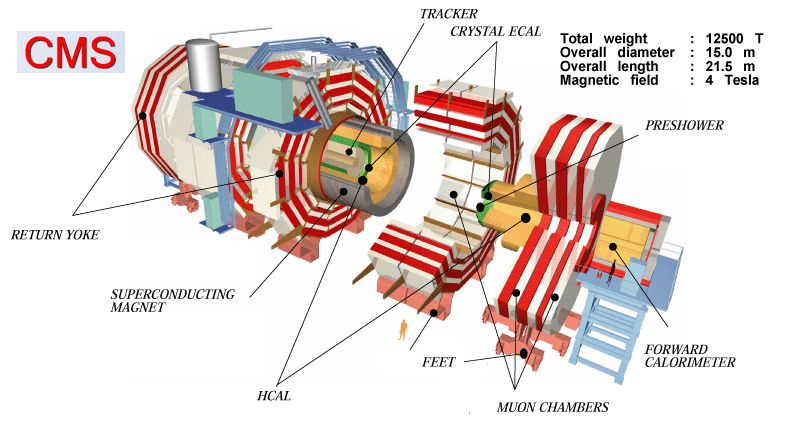
\includegraphics[width=0.90\linewidth]{Experiment/CMS/Image/cmsdiag.png}
	  \caption{Diagram of the CMS detector \cite{cmsDiagram}. Various parts 
	  of the CMS detector are shown starting from tracker to ECAL to HCAL to magnet to 
	  the muon chambers.}
  \label{fig:cms_diag}
  \end{center}
\end{figure}
%Fig\pdfcomment[author={FIG COURTESY}]{http://physics.stackexchange.com/questions/139540/how-detectors-in-particle-colliders-can-differentiate-neutrons-from-antineutrons}}
\begin{figure}
  \begin{center}
  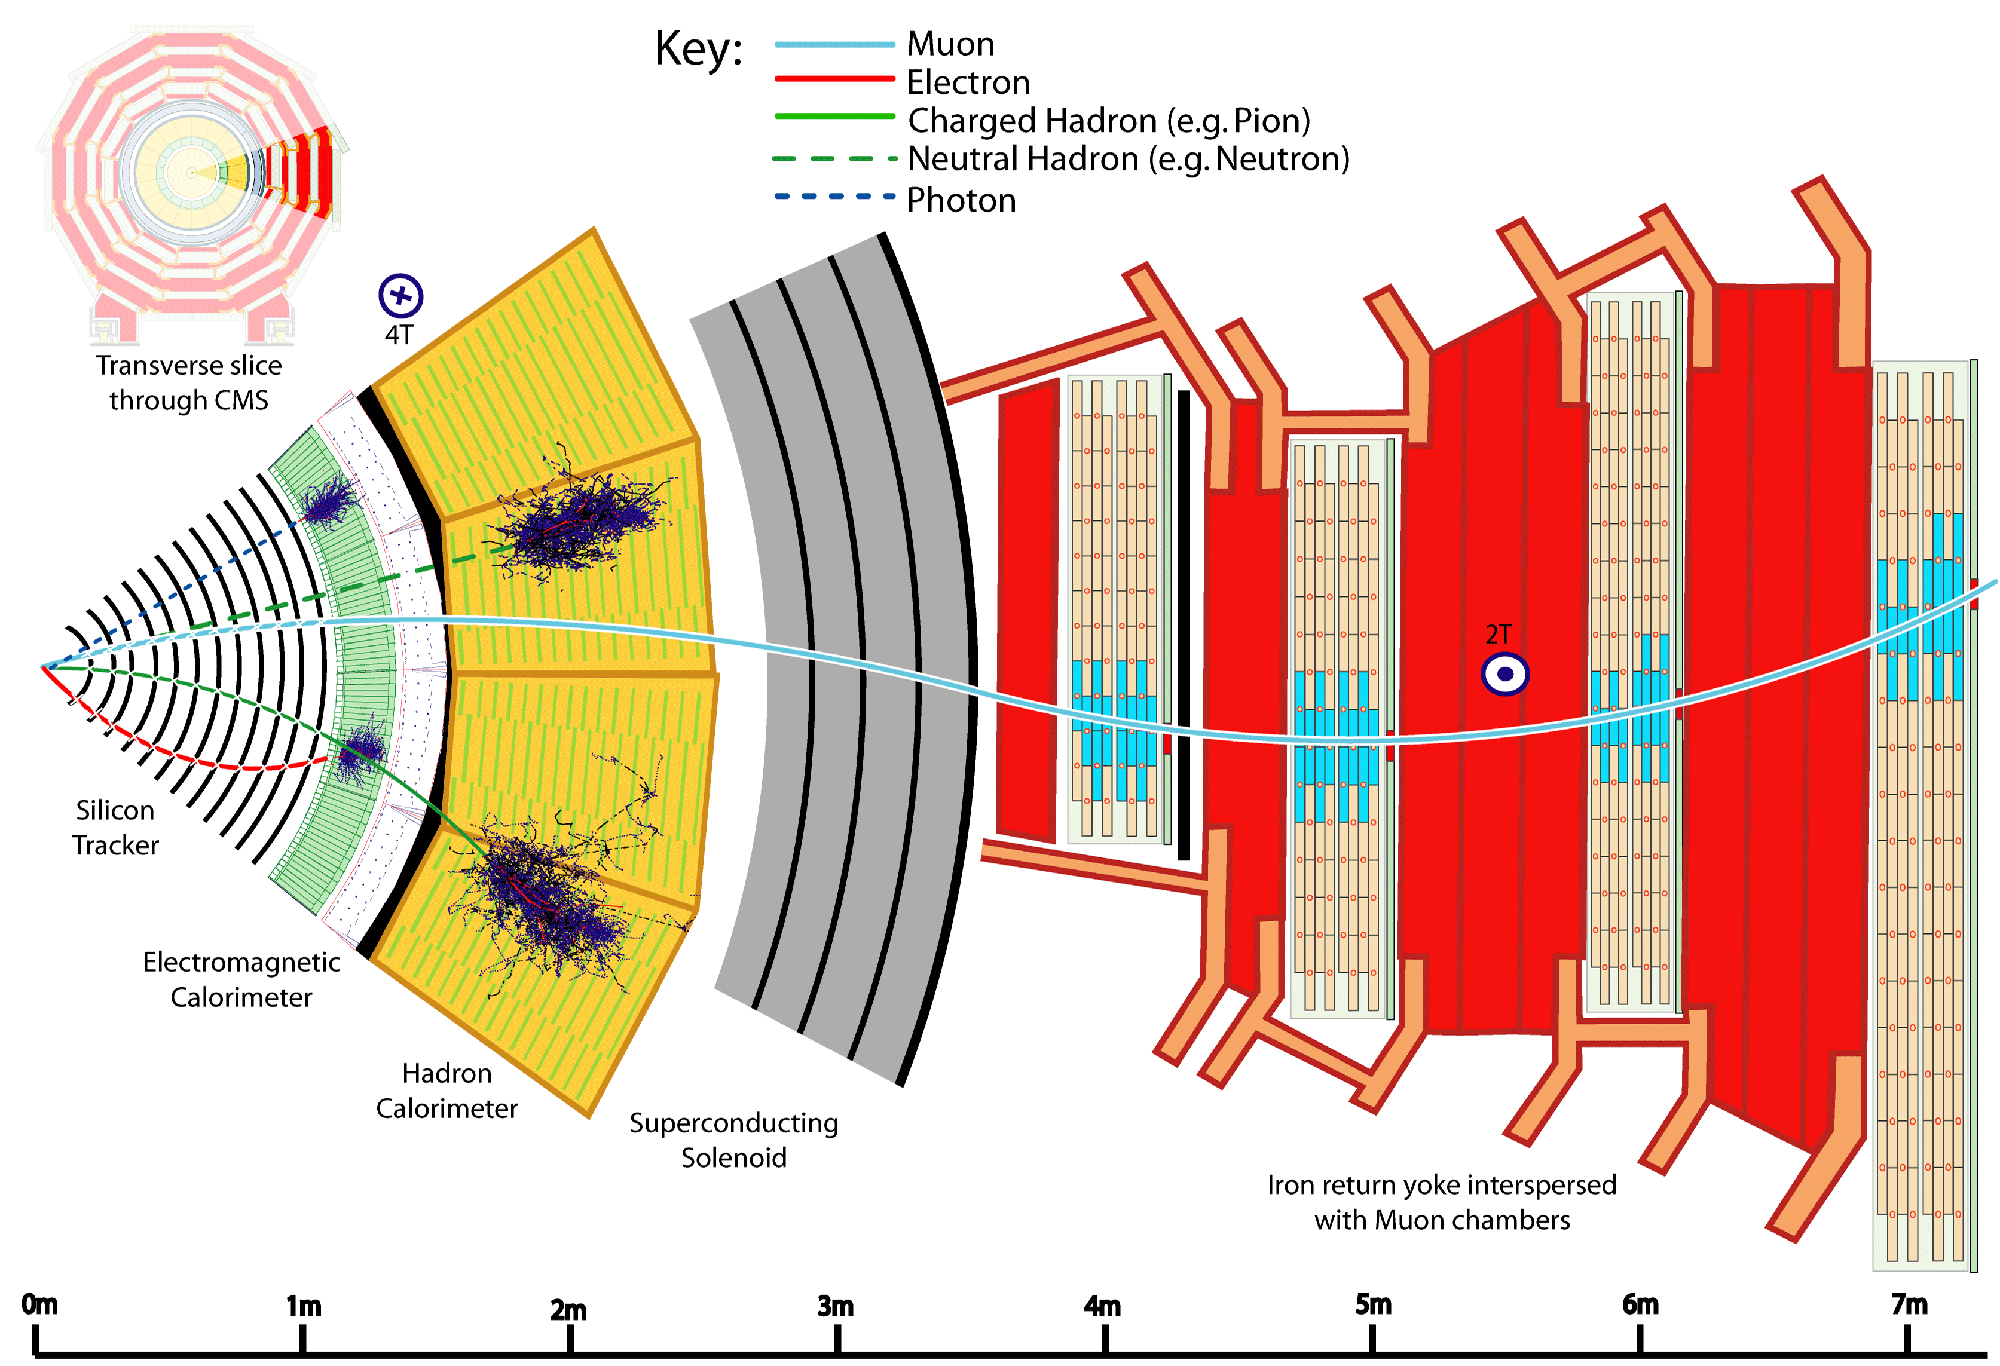
\includegraphics[width=0.90\linewidth]{Experiment/CMS/Image/cmstrack.png}
	  \caption{Trajectories of various particles inside the CMS detector 
	  \cite{Sirunyan:2270046}. The charged particles
	  such as electrons, muons, and charged pions ($\pi^\pm$) are bent inside and 
	  outside the
	  solenoid whereas the neutral particles such as photons and neutral pions ($\pi^0$)
	  traverse without being bent. The silicon tracker is mainly for measuring
	  the momentum of particles whereas the ECAL and HCAL measure the 
	  energy deposits. The electrons and photons deposit their energy inside the 
	  ECAL whereas the hadrons deposit in both ECAL and HCAL. The muons are the
	  only particles that traverses all the way to the muon chambers.}
  \label{fig:cms_track}
  \end{center}
\end{figure}
